{{%Localize command definitions

\newcommand{\NN}{\mathbb{N}}
\renewcommand{\implies}{\Rightarrow}
\newcommand{\implied}{\Leftarrow}
\newcommand{\eps}{\varepsilon}
\newcommand{\gfp}{\mathrm{gfp}}
\newcommand{\lfp}{\mathrm{lfp}}
\newcommand{\defas}{\coloneqq}
\renewcommand{\le}{\sqsubseteq}
\renewcommand{\ge}{\sqsupseteq}
\renewcommand{\sqcap}{\bigsqcap}
\renewcommand{\sqcup}{\bigsqcup}
\newcommand{\bottom}{\perp}


\newcommand{\Theorem}[2][]{\begin{theorem}[#1]#2\end{theorem}}
\newcommand{\Definition}[2][]{\begin{definition}[#1]#2\end{definition}}
\newcommand{\Example}[2][]{\begin{example}[#1]#2\end{example}}
\newcommand{\Homework}[2][]{\begin{homework}[#1]#2\end{homework}}
\newcommand{\Lemma}[2][]{\begin{lemma}[#1]#2\end{lemma}}
\newcommand{\Remark}[2][]{\begin{remark}[#1]#2\end{remark}}
\newcommand{\Figure}[1]{\begin{figure}#1\end{figure}}
\newcommand{\Itemize}[1]{\begin{itemize}#1\end{itemize}}
\newcommand{\Enumerate}[1]{\begin{enumerate}#1\end{enumerate}}

\usetikzlibrary {petri}

\chapter{Class 22}

Calculus of Communicating Sysfems (CCS) can be given two semantics.
\Itemize {
	\item \emph{Sequential.} 
		Labeled transition systems and logics (e.g., Hennessy-Milner logic (HML) and temporal logic)
	\item \emph{Truly concurrent.} 
		Parallelism is different from nondeterminism.
		Uses Petri nets.
}
	

\Definition[Petri nets]{
	A \emph{petri net} is a tuple $N = (P, T)$ where $P$ is a set of places and $T$ a set of transitions.
	The state of a petri net is given by a marking $M \colon P \to \NN$ and a transition is a function that takes a marking and an action and returns another marking, i.e., $t \colon M \to M$.
	Equivalently, considering a set of names for each transition (actions) $A$, we have that $T \colon M \times A \to M$.
}

\Remark[Petri nets as lebeled transition systems] {
	A Petri net $N = (P, T)$ can be interpreted as the following labeled transition system (LTS) $LTS_N = (M, \to)$.
	The transition $\to$ is given by $m \to m'$ if and only if there exists $t \in T$ such that 
	\Itemize {
		\item the transformation $t$ decomposes in precodition $^*t \in M$, action $a \in A$ and postcondition $t^* \in M$, i.e., $t = (^*t, a, t^*)$.
		\item the precodition $^*t$ is contained in $m$, i.e., $^*t \subseteq m$.
		\item the transformation $t$ converts $m$ into $m'$, i.e., $m' = m - ^*t + t^*$.
	}

}

\Example[Petri net] {
	Consider the Petri net $N = (P, T)$ where $P = \{ p_1, p_2, p_3, p_4, p_5 \}$, $T = \{ t \}$, and $t \colon \{ (p_1, 2), (p_2, 1) \} \mapsto \{ (p_4, 1), (p_5, 1) \}$.
	In other words, $t$ can fire a transition if there are $2$ markings in $p_1$ and $1$ marking in $p_2$, and adds $1$ marking in $p_4$ and $1$ marking in $p_5$.  
}
\Figure { 
	\centering
	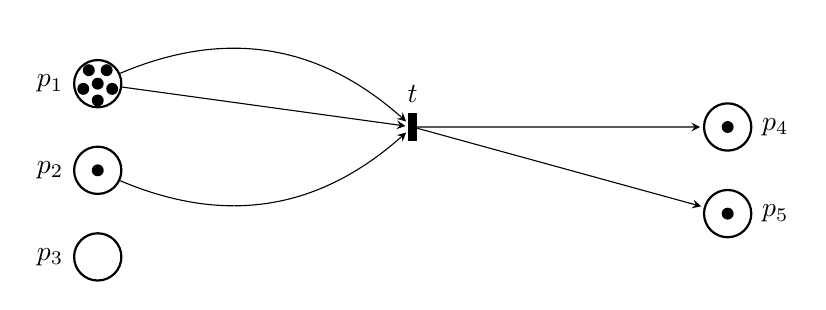
\begin{tikzpicture}[
		yscale=-1.1,
		thin,
		>=stealth,
  		every transition/.style={fill,minimum width=1mm,minimum height=3.5mm},
  		every place/.style={draw,thick,minimum size=6mm}
	]

		% Places
		\node[place,label=left:$p_1$] (p1) at (0, 1) {};    
		\node[place,label=left:$p_2$] (p2) at (0, 2) {};    
		\node[place,label=left:$p_3$] (p3) at (0, 3) {};    
		\node[place,label=right:$p_4$] (p4) at (8, 1.5) {};    
		\node[place,label=right:$p_5$] (p5) at (8, 2.5) {};  

		% Tokens
		\node[token, tokens=5] at (p1) {}; 
		\node[token] at (p2) {};
		\node[token] at (p4) {};  
		\node[token] at (p5) {};  

		% Transitions
		\node[transition, label=above:$t$] at (4, 1.5) {}  
			edge[] [pre] (p1) 
			edge[bend left] [pre] (p1) 
			edge[bend right] [pre] (p2) 
			edge [post] (p4)
			edge [post] (p5);
	\end{tikzpicture}
	\caption{Petri net example}
}

\Definition[Sequenctial nets]{
	A Petri net is \emph{sequential} if all transformations $t$ have a precondition $^*t$ such that $|^*t| \le 1$.
	Sequential nets are equivalent to regular laguages for finite strings. 
}


\Figure {
	\centering
	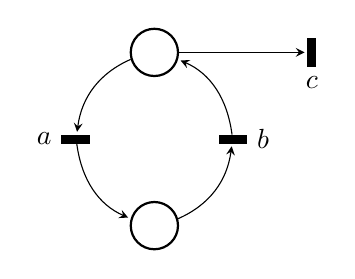
\begin{tikzpicture}[
		yscale=-1.1,
		thin,
		>=stealth,
  		every transition/.style={fill,minimum width=1mm,minimum height=3.5mm},
  		every place/.style={draw,thick,minimum size=6mm}
	]

		% Places
		\node[place] (p1) at (1, 0) {};    
		\node[place] (p2) at (1, 2) {};

		% Transitions
		\node[transition, label=left:$a$, style={fill,minimum width=3.5mm,minimum height=1mm}] at (0, 1) {}  
			edge[bend right] [pre] (p1)
			edge[bend left] [post] (p2);
		\node[transition, label=right:$b$, style={fill,minimum width=3.5mm,minimum height=1mm}] at (2, 1) {}  
			edge[bend right] [pre] (p2)
			edge[bend left] [post] (p1);
		\node[transition, label=below:$c$] at (3, 0) {}  
			edge[] [pre] (p1);
	\end{tikzpicture}
	\caption{Sequential net example}
}

\Definition[Basic parallel processes]{
	A Petri net is a \emph{basic parallel processes} if all transformations $t$ have a precondition $^*t$ such that $|^*t| = 1$.
	Basic parallel processes are equivalent to context-free languages for finite strings. 
}

\Figure {
	\centering
	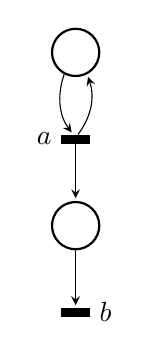
\begin{tikzpicture}[
		yscale=-1.1,
		thin,
		>=stealth,
  		every transition/.style={fill,minimum width=3.5mm,minimum height=1mm},
  		every place/.style={draw,thick,minimum size=6mm}
	]

		% Places
		\node[place] (p1) at (0, 0) {};    
		\node[place] (p2) at (0, 2) {};

		% Transitions
		\node[transition, label=left:$a$] at (0, 1) {}  
			edge[bend right] [pre] (p1)
			edge[] [post] (p2)
			edge[bend left] [post] (p1);
		\node[transition, label=right:$b$] at (0, 3) {}  
			edge[] [pre] (p2);
	\end{tikzpicture}
	\caption{Basic parallel process example}
}

\Definition[Chomsky hierarchy] {
	The \emph{Chomsky hierarchy} is a hierarchy of sequential computation given by
	\[
		FA 
			\subseteq PDA
			\subseteq LBA
			\subseteq TM \,,
	\]
	where the decidabilities are as follows.
	\Itemize {
		\item FA. Fully decidable.
		\item PDA. Universality is undecidable, i.e., $L(A) \stackrel{?}{=} \Sigma^*$.
		\item LBA. Emptyness is undecidable, i.e., $L(A) \stackrel{?}{=} \emptyset$.
		\item TM. Membership is undecidable, i.e., $w \stackrel{?}{\in} L(A)$.
	}
}

\Definition[Concurrency hierarchy] {
	The \emph{concurrency hierarchy} is a hierarchy of concurrent computation given by
	\[
		FA 
			\subseteq BPP
			\subseteq CCS
			\subseteq TM \,,
	\]
	where, in CCS, reachability is decidable but non-elementary.
}

\Homework[Ortogonal hierarchies]{
	Solve the following tasks.
	\Enumerate {
		\item Show that $X = a (X | b) + c (X | d) + e$ is not context-free.
		Hint: use the pumping lemma.

		\item Present a context-free language that is not in BPP, and try to prove it. 
	}
}

\Definition[Coverage problem for Petri nets] {
	Given a Petrin net $N$ and two marking $m, m'$, the problem is to decide the existence of a sequence of transitions that take $m$ to a marking that covers $m'$, i.e., if there exists $m*$ such that $m \to m*$ and $m' \subseteq m*$.
}

\Remark {
	As opposed to the reachability question, the coverage problem asks for $m' \subseteq m*$ instead of $m' = m*$.
}

The coverage problem is a finite problem, since every finite Petri net $N$ has a finite coverage tree of size $\mathcal{O}(n^n)$ where $n = |N|$.
The coverage tree can be obtained by the Karp-Miller algorithm, which generates a tree of depth at most $\mathcal{O}(n \log n)$.

Consider the Petri net with an initial marking is given in \Cref{Figure: Karp-Miller Petri net}.
The corresponding coverage tree is given in \Cref{Figure: Karp-Miller coverage tree}.
Note that $m'$ is covered by $m$ if there is a node in the tree that covers it. 

\Figure {
	\centering
	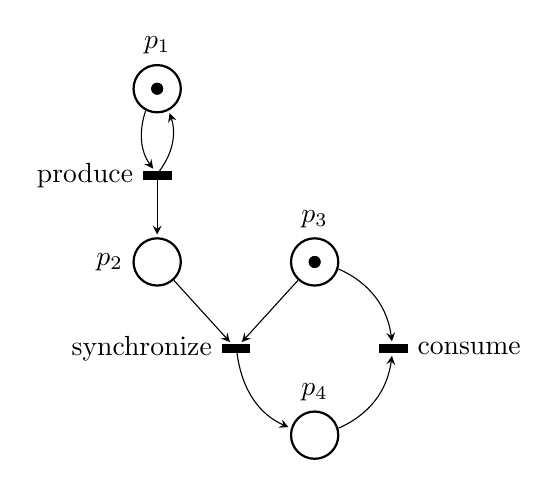
\begin{tikzpicture}[
		yscale=-1.1,
		thin,
		>=stealth,
  		every transition/.style={fill,minimum width=3.5mm,minimum height=1mm},
  		every place/.style={draw,thick,minimum size=6mm}
	]

		% Places
		\node[place, label=above:$p_1$] (p1) at (0, 0) {};    
		\node[place, label=left:$p_2$] (p2) at (0, 2) {};   
		\node[place, label=above:$p_3$] (p3) at (2, 2) {};   
		\node[place, label=above:$p_4$] (p4) at (2, 4) {};

		% Tokens
		\node[token, tokens=1] at (p1) {}; 
		\node[token, tokens=1] at (p3) {};

		% Transitions
		\node[transition, label=left:{produce}] at (0, 1) {}  
			edge[bend right] [pre] (p1)
			edge[bend left] [post] (p1)
			edge[] [post] (p2);
		\node[transition, label=left:{synchronize}] at (1, 3) {}  
			edge[] [pre] (p2)
			edge[] [pre] (p3)
			edge[bend left] [post] (p4);
		\node[transition, label=right:{consume}] at (3, 3) {}  
			edge[bend right] [pre] (p4)
			edge[bend left] [pre] (p3);
	\end{tikzpicture}
	\caption{Karp-Miller Petri net with initial configuration example}
	\label{Figure: Karp-Miller Petri net}
}
\Figure {
	\centering
	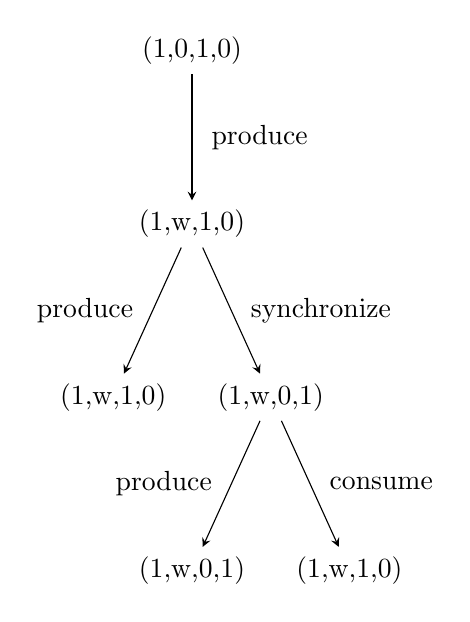
\begin{tikzpicture}[
		yscale=-1.1,
		thin,
		>=stealth,
	]

		% markings
		\node (a) at (0, 0) {(1,0,1,0)};
		\node (b) at (0, 2) {(1,w,1,0)};    
		\node (c) at (-1, 4) {(1,w,1,0)};   
		\node (d) at (1, 4) {(1,w,0,1)};
		\node (e) at (0, 6) {(1,w,0,1)};
		\node (f) at (2, 6) {(1,w,1,0)};

		% transformations
		\path [->] (a) edge node[label=right:{produce}] {} (b);
		\path [->] (b) edge node[label=left:{produce}] {} (c);
		\path [->] (b) edge node[label=right:{synchronize}] {} (d);
		\path [->] (d) edge node[label=left:{produce}] {} (e);
		\path [->] (d) edge node[label=right:{consume}] {} (f);
	\end{tikzpicture}
	\caption{Karp-Miller coverage tree}
	\label{Figure: Karp-Miller coverage tree}
}

\Definition[Control-flow models] {
	Graphs whose nodes represent control states and whose edges represent control flow. 
	For example, labeled transition systems and Petri nets.
}

\Definition[Data-flow models] {
	Also called circuits, they are graphs whose nodes represent actors (gates) and whose edges represent data flow. 
}

\Cref{Figure: Data-flow model} represents a data-flow model.

\Figure {
	\centering
	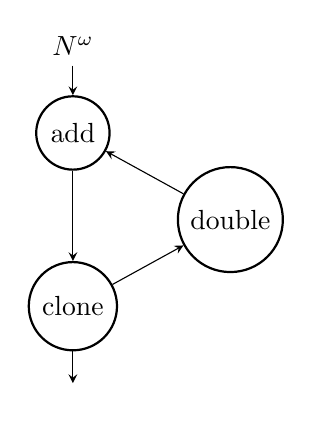
\begin{tikzpicture}[
		yscale=-1.1,
		thin,
		>=stealth,
	]

		% markings
		\node (input) at (0, 0) {$\NN^\omega$};
		\begin{scope}[every node/.style={circle,thick,draw}]
			\node (b) at (0, 1) {add};    
			\node (c) at (0, 3) {clone};   
			\node (d) at (2, 2) {double};
		\end{scope}
		\node (output) at (0, 4) {};

		% transformations
		\path [->] (input) edge node {} (b);
		\path [->] (b) edge node {} (c);
		\path [->] (c) edge node {} (d);
		\path [->] (d) edge node {} (b);
		\path [->] (c) edge node {} (output);
	\end{tikzpicture}
	\caption{Data-flow model example}
	\label{Figure: Data-flow model}
}

\Definition[Combinatorial circuits] {
	A data-flow model is a \emph{combinatorial circuit} if there are no loops.
	For combinatorial circuits, every tuple of inputs produces a tuple of outputs.
}
\Definition[Sequential circuits] {
	A data-flow model is a \emph{sequential circuit} if there are loops.
	For sequential circuits, every sequence of inputs produces a sequence of outputs.
}

To deal with loops in sequential circuits, there are two approaches:
\Itemize {
	\item synchronous (clocked); and
	\item asynchronous (queues as channels).
}

% Control flow and data flow


}} % End localization of command definitions
